% ------------------------------------------------------------------------------
\cleardoublepage
% ------------------------------------------------------------------------------
\chapter{A fejlesztői környezet bemutatása}
% ------------------------------------------------------------------------------

Ebben a fejezetben be fogom mutatni, hogy milyen környezetben dolgoztam a
fejlesztés során. Kitérek arra, hogy a forrásfájlokat milyen környezetben
tároltam. Megmutatom, hogy milyen szkripteket fejlesztettem, melyek
elősegítették a hibák kiküszöbölését, a dokumentumok fordítását és a kódbázis
bővítését is.

% ------------------------------------------------------------------------------
\section{Git: a verziókezelő rendszer}
% ------------------------------------------------------------------------------

A szoftverfejlsztés világában a \textit{git} rendszer egyre inkább alapvető
eszközzé válik. A \textit{git} nemcsak egy egyszerű verziókezelő rendszer,
hanem egy olyan eszköz is, amely újradefiniálja a fejlesztők munkamódszereit,
hiszen jelentős előnyöket nyújt a projektmenedzsment és a csapatmunka terén.

% ------------------------------------------------------------------------------
\subsection{Út a git megjeleéséig}
% ------------------------------------------------------------------------------

Mi is az a verziókezelés, és miért is olyan fontos? A verziókezelés egy olyan
rendszer, amely lehetővé teszi, hogy egy adott dokumentum, vagy fájl
változásainak időben nyomon követését. Ezt a módszert általában szoftverek
forrásfájljainak nyilvántartására használják, de valójában egy számítógépen
található bármilyen típusú fájlra alkalmazható.

Sok embernél a verziókezelés abban merül ki, hogy a fájlokat egy másik
könyvtárba másolják, és a fájlok nevéhez egy sorszámot fűznek. Ez a megközelítés
rendkívül elterjedt, de sajnos nem túl hatékony, és még hibaérzékeny is. Könnyű
elfeledkezni arról, hogy melyik fájl melyik verzióját melyik könyvtárban
találhatjuk meg. Előfordulhat ezáltal, hogy egy régebbi verzióval dolgozunk,
vagy éppen egy másik fejlesztő munkáját írjuk felül.

\begin{figure}[htb]
	\centering
	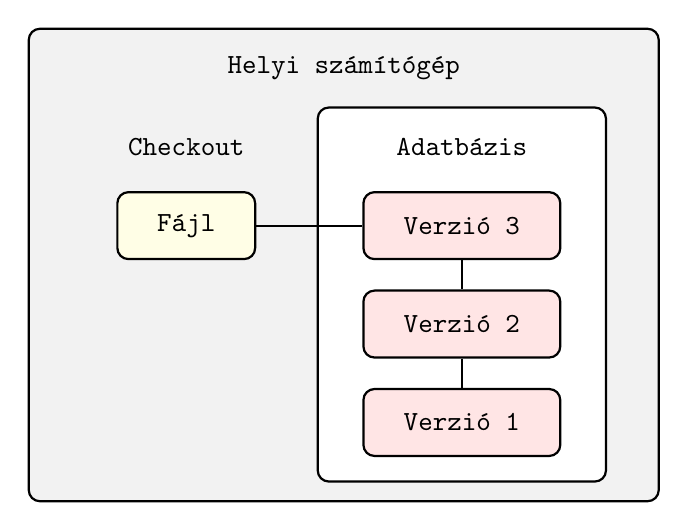
\begin{tikzpicture}[thick]
		\draw[rounded corners, fill=gray!10] (-4,-3) rectangle (4,3);
		\draw[rounded corners, fill=white] (-0.33,-2.75) rectangle (3.33,2);


		\node at (0, 2.5) {\texttt{Helyi számítógép}};

		\node at (-2,1.5) {\texttt{Checkout}};
		\node[
			rectangle, rounded corners, fill=yellow!10, draw=black,
			minimum width=1.75cm, minimum height=0.85cm
		] (F) at (-2,0.5) {\texttt{Fájl}};

		\node at (1.5, 1.5) {\texttt{Adatbázis}};

		\node[
			rectangle, rounded corners, fill=red!10, draw=black,
			minimum width=2.5cm, minimum height=0.85cm
		] (V3) at (1.5,0.5) {\texttt{Verzió 3}};
		\node[
			rectangle, rounded corners, fill=red!10, draw=black,
			minimum width=2.5cm, minimum height=0.85cm
		] (V2) at (1.5,-0.75) {\texttt{Verzió 2}};
		\node[
			rectangle, rounded corners, fill=red!10, draw=black,
			minimum width=2.5cm, minimum height=0.85cm
		] (V1) at (1.5,-2) {\texttt{Verzió 1}};

		\draw (F) -- (V3) -- (V2) -- (V1);
	\end{tikzpicture}
	\caption{Helyi verziókezelő renszerek felépítése \cite{git_scm_1.1}}
	% \label{fog:fig:local-vcs}
\end{figure}

Ennek a problémának az orvosolására a programozók már régen kifejlesztettek
helyi verziókezelő rendszereket, amelyek mögött egy egyszerű adatbázis állt.
Az egyik legnépszerűbb ilyen eszköz az \textit{RCS} (Revision Control System --
Revíziós Ellenőrzési Rendszer) volt, amely a mai napig számtalan Unix rendszeren
elérhető. Az RCS egy egyszerű rendszer, amely a fájlok mentéséhez \textit{diff}
fájlokat használ. A \textit{diff} fájlokban csak azok a sorok szerepelnek,
amelyek változtak, így ezen fájlok mérete kicsi marad. \cite{rcs_documentation}

% https://cvs.nongnu.org

\begin{figure}[htb]
	\centering
	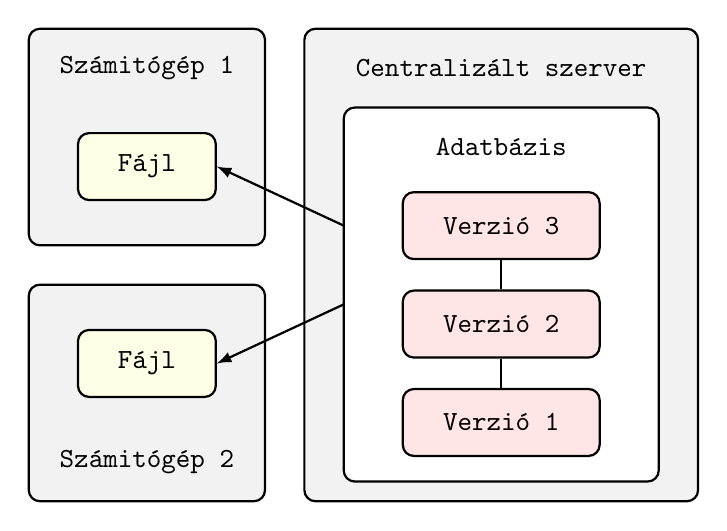
\begin{tikzpicture}[thick]
		\draw[rounded corners, fill=gray!10] (-4,-3) rectangle ++(3,2.75);
		\draw[rounded corners, fill=gray!10] (-4,0.25) rectangle ++(3,2.75);
		\draw[rounded corners, fill=gray!10] (-0.5,-3) rectangle ++(5,6);
		\draw[rounded corners, fill=white] (0,-2.75) rectangle (4,2);

		\node (C1) at (-2.5,2.5) {\texttt{Számitógép 1}};
		\node (C2) at (-2.5,-2.5) {\texttt{Számitógép 2}};

		\node[
			rectangle, rounded corners, fill=yellow!10, draw=black,
			minimum width=1.75cm, minimum height=0.85cm
		] (F1) at (-2.5,1.25) {\texttt{Fájl}};
		\node[
			rectangle, rounded corners, fill=yellow!10, draw=black,
			minimum width=1.75cm, minimum height=0.85cm
		] (F2) at (-2.5,-1.25) {\texttt{Fájl}};

		\node at (2,2.5) {\texttt{Centralizált szerver}};
		\node at (2, 1.5) {\texttt{Adatbázis}};

		\node[
			rectangle, rounded corners, fill=red!10, draw=black,
			minimum width=2.5cm, minimum height=0.85cm
		] (V3) at (2,0.5) {\texttt{Verzió 3}};
		\node[
			rectangle, rounded corners, fill=red!10, draw=black,
			minimum width=2.5cm, minimum height=0.85cm
		] (V2) at (2,-0.75) {\texttt{Verzió 2}};
		\node[
			rectangle, rounded corners, fill=red!10, draw=black,
			minimum width=2.5cm, minimum height=0.85cm
		] (V1) at (2,-2) {\texttt{Verzió 1}};

		\draw (V3) -- (V2) -- (V1);
		\draw [-latex] (0,.5) -- (F1.east);
		\draw [-latex] (0,-.5) -- (F2.east);
	\end{tikzpicture}
	\caption{Centralizált verziókezelő renszerek felépítése \cite{git_scm_1.1}}
	% \label{fog:fig:local-vcs}
\end{figure}

Az \textit{RCS} egy egyszerű, és hatékony rendszernek bizonyult, viszont volt
egy nagyon fontos hiányossága. A rendszer nem támogatta a többfejlesztői
munkát. Ennek a problémának az orvosolására fejlesztették ki a centralizált
verziókezelő rendszereket. Az ilyen rendszerek esetén (mint pl. a \textit{CVS}
(Concurrent Versions System -- Egyidejű verziók rendszere)) egy központi
szerver tárolja a fájlokat, és a fejlesztők a szerveren keresztül tudják
elérni a fájlokat. Egy ilyen rendszer használata számos előnnyel jár a helyi
rendszerekkel szemben, viszont van egy súlyos hibája, amely a központi
szerverben rejlik. Ha a szerver egy pár órára leáll, akkor senki sem tud
dolgozni. Ha a szerver a fájlokat tároló adathordozóval együtt elromlik,
az az adatok és történetük elvesztését jelenti. \cite{cvs_documentation}

\begin{figure}[htb]
	\centering
	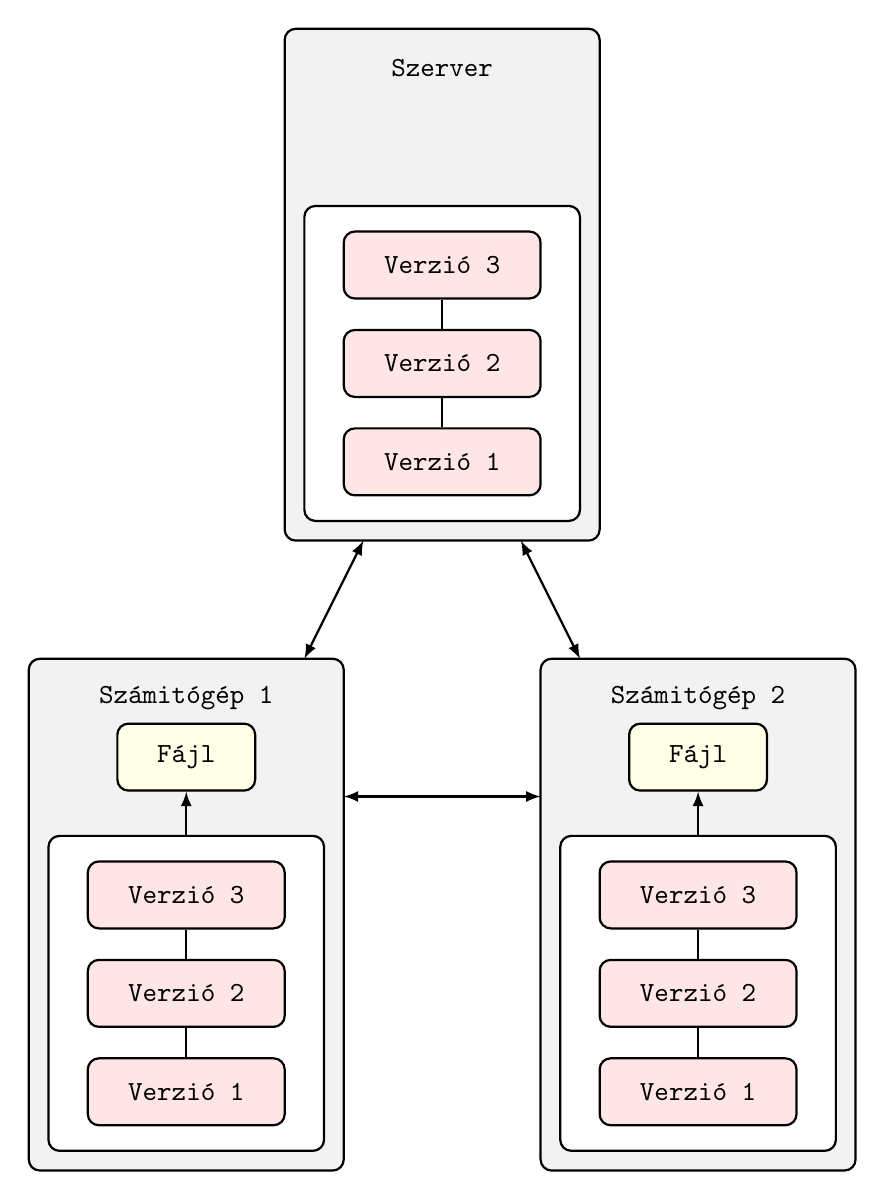
\begin{tikzpicture}[thick]
		\foreach \x/\y in {0/0,-1/-1,1/-1} {
				\begin{scope}[xshift=\x*3.25cm, yshift=\y*8cm]
					\draw[rounded corners, fill=gray!10] (2,3) rectangle ++(-4,-6.5);
					\draw[rounded corners, fill=white] (1.75,0.75) rectangle ++(-3.5,-4);

					\node[
						rectangle, rounded corners, fill=red!10, draw=black,
						minimum width=2.5cm, minimum height=0.85cm
					] (V3) at (0,0) {\texttt{Verzió 3}};
					\node[
						rectangle, rounded corners, fill=red!10, draw=black,
						minimum width=2.5cm, minimum height=0.85cm
					] (V2) at (0,-1.25) {\texttt{Verzió 2}};
					\node[
						rectangle, rounded corners, fill=red!10, draw=black,
						minimum width=2.5cm, minimum height=0.85cm
					] (V1) at (0,-2.5) {\texttt{Verzió 1}};

					\draw (V3) -- (V2) -- (V1);
				\end{scope}
			}

		\node (S) at (0,2.5) {\texttt{Szerver}};

		\node (C1) at (-3.25,-5.5) {\texttt{Számitógép 1}};
		\node (C2) at (3.25,-5.5) {\texttt{Számitógép 2}};
		\node[
			rectangle, rounded corners, fill=yellow!10, draw=black,
			minimum width=1.75cm, minimum height=0.85cm
		] (F1) at (-3.25,-6.25) {\texttt{Fájl}};
		\node[
			rectangle, rounded corners, fill=yellow!10, draw=black,
			minimum width=1.75cm, minimum height=0.85cm
		] (F2) at (3.25,-6.25) {\texttt{Fájl}};

		\draw [-latex] (-3.25,-7.25) -- (F1);
		\draw [-latex] (3.25,-7.25) -- (F2);

		\draw [latex-latex] (-1.25,-6.75) -- (1.25,-6.75);
		\draw [latex-latex] (-1.75,-5) -- (-1,-3.5);
		\draw [latex-latex] (1.75,-5) -- (1,-3.5);
	\end{tikzpicture}
	\caption{Centralizált verziókezelő renszerek felépítése \cite{git_scm_1.1}}
	% \label{fog:fig:local-vcs}
\end{figure}

Itt jönnek képbe a elosztott verziókezelő rendszerek, mint pl. a \textit{git}.
Ilyen rendszereknél a felhasználók nemcsak a fájlok legfrisebb verzióját
birtokolják, hanem teljes mértékben lemásolják az összes adatot, beleértve
a fájlokat, és azok teljes történetét is. Ez a megközelítés sokkal
biztonságosabb, mint a centralizált rendszereké, hiszen ha egy szerver
elromlik, akkor a fájlok másolatai még mindig elérhetőek. Ráadásul a legtöbb
ilyen rendszer jól kezeli, ha egy projekten belül több tárolóhelyet szeretnénk
használni. Ez a kedvező tulajdonság olyan munkafolyamatokat is lehetővé
tesz, amelyek centralizált rendszerekben nem megoldhatóak, például
hierarchikus modellek alkalmazását.\cite{git_scm_1.1}

% ------------------------------------------------------------------------------
\subsection{A git rövid története}
% ------------------------------------------------------------------------------

A \textit{Linux kernel} egy nagyszabású, nyílt forráskódú projet. A kezdeti
időszakban a szoftver módosításait javítások és archivált fájlok formájában
adták tovább. 2002-ben a \textit{Linux kernel projekt} egy \textit{BitKeeper}
nevű, elosztott verziókezelő rendszerre tért át. 2005-ben a \textit{Linux}
fejlesztői és a \textit{BitKeeper} mögött álló cég közötti kapcsolat egyre
inkább leépült, a \textit{BitKeeper} szoftver ingyenes használata pedig
megszűnt. Ekkor a \textit{Linux} fejlesztői úgy döntöttek, hogy saját
verziókezelő rendszert fejlesztenek, amely a \textit{BitKeeper} által
használt adatmodellt követi. A projektet Linus Torvalds vezette, és a
\textit{git} nevet kapta. Az új rendszer készítése során az alábbi célokat
tartották szem előtt:
\begin{itemize}
	\item gyorsaság,
	\item egyszerűség,
	\item támogassa a nemlineáris fejlesztést,
	\item teljesen elosztott legyen,
	\item támogassa a nagy projekteket is
\end{itemize}
Az első megjelenés óta a \textit{git} nagyon sokat fejlődött, viszont a fenti
célok mindvégig megmaradtak, mára pedig a legelterjedtebb verziókezelő rendszer
lett. \cite{git_scm_1.2}

% ------------------------------------------------------------------------------
\subsection{Az alapok}
% ------------------------------------------------------------------------------

Egy \textit{git} alapú verziókezelő rendszer használata nagyon egyszerű.
Ha egy már meglévő projektet szeretnénk egy \textit{git} alapú rendszerbe
helyezni, akkor a következő parancsot kell kiadnunk:

\begin{lstlisting}[caption={A git inicializálása},language=sh]
  $ cd <projekt könyvtár> # A projekt könyvtárba navigálunk
  $ git init              # A projekt könyvtár verziókezelését inicializáljuk
\end{lstlisting}

A parancs hatására a könyvtárban létrejött egy \texttt{.git} nevű rejtett
mappa, amely tartalmazza a \textit{git} számára alapvető fájlokat.
Ezt a folyamatot a \textit{git repository} inicializálásának nevezzük.
Fontos, hogy ilyenkor a projetben található fájlok nem lesznek
automatikusan verziókezelve, hanem úgynevezett \texttt{untracked} állapotba
kerülnek. Ez azt jelenti, hogy a \textit{git} nem fogja nyomon követni a
fájlok változásait. Ahhoz, hogy egy fájlt a \textit{git} nyomon kövessen,
a következő parancsot kell kiadnunk:

\begin{lstlisting}[caption={Fájlok hozzáadása},language=sh]
  $ git add <fájl neve>
\end{lstlisting}

Ekkor a fájlok \texttt{staged} állapotba kerülnek, vagyis a következő
pillanatképbe bekerülnek. Ahhoz, hogy egy pillanatképet készítsünk a
projekt állapotáról, a következő parancsot kell kiadnunk:

\begin{lstlisting}[caption={Pillanatkép mentése},language=sh]
  $ git commit -m "A commit üzenet"
\end{lstlisting}

A parancs hatására a \textit{git} létrehoz egy pillanatképet a projekt
állapotáról, és a pillanatképhez hozzárendeli a megadott üzenetet. Az ebben
szereplő fájlok pedig \texttt{tracked}, vagyis nyomon követett állapotba
kerülnek. Amennyiben a fájlok módosulnak, úgy a \textit{git} automatikusan
\texttt{modified} állapotba helyezi őket. Ha a módosításokat menteni
szeretnénk, akkor a fenti parancsokat kell újra kiadnunk. A \texttt{git add}
parancs hatására a fájlok \texttt{staged} állapotba kerülnek, majd a
\texttt{git commit} parancs hatására a fájlok pillanatképe elkészül.
Az előbb leírt folyamatot a \ref{fig:git-lifecycle} ábra szemlélteti.

\begin{figure}[htb]
	\centering
	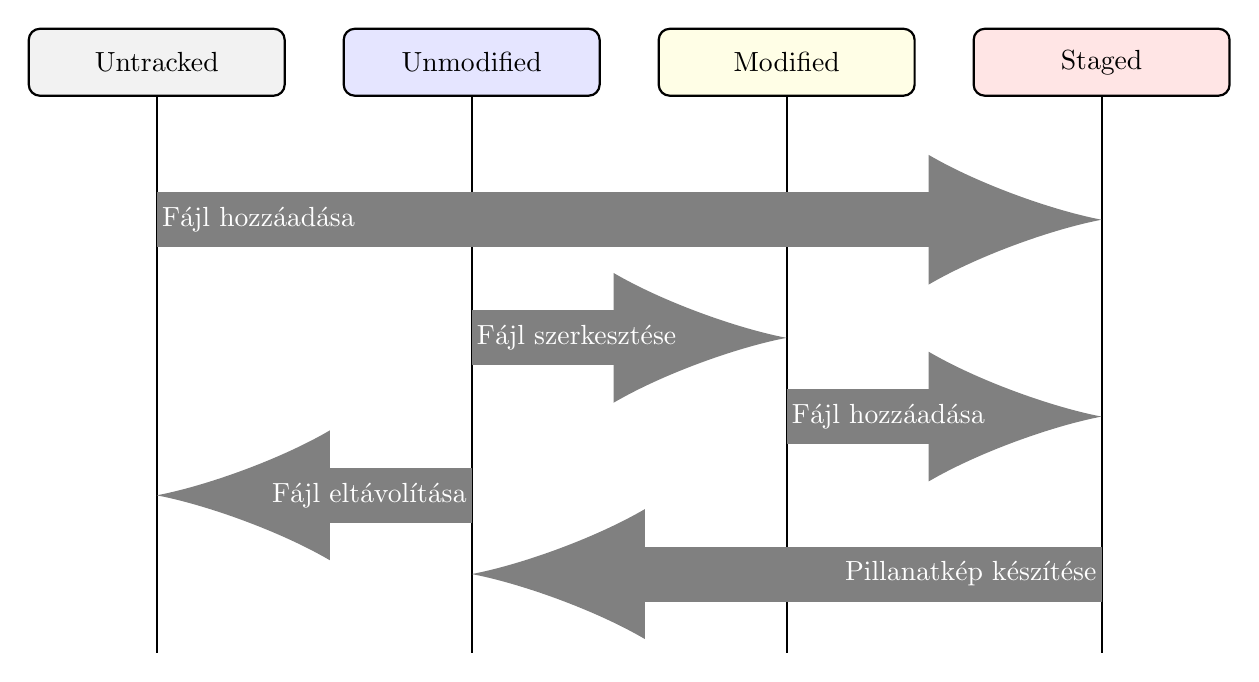
\begin{tikzpicture}[thick]
		\node[
			rectangle, rounded corners, fill=gray!10, draw=black,
			minimum width=3.25cm, minimum height=0.85cm
		] (U) at (-6, 0) {Untracked};
		\node[
			rectangle, rounded corners, fill=blue!10, draw=black,
			minimum width=3.25cm, minimum height=0.85cm
		] (X) at (-2, 0) {Unmodified};
		\node[
			rectangle, rounded corners, fill=yellow!10, draw=black,
			minimum width=3.25cm, minimum height=0.85cm
		] (M) at (2, 0) {Modified};
		\node[
			rectangle, rounded corners, fill=red!10, draw=black,
			minimum width=3.25cm, minimum height=0.85cm
		] (A) at (6, 0) {Staged};

		\foreach \l in {U,X,M,A} {
				\draw (\l) -- ++(0,-7.5);
			}

		\draw[-latex, line width=7mm, draw=gray] (-6,-2) -- (6,-2)
		node[right=-4mm, white, pos=0] {Fájl hozzáadása};
		\draw[-latex, line width=7mm, draw=gray] (-2,-3.5) -- (2,-3.5)
		node[right=-4mm, white, pos=0] {Fájl szerkesztése};
		\draw[-latex, line width=7mm, draw=gray] (2,-4.5) -- (6,-4.5)
		node[right=-4mm, white, pos=0] {Fájl hozzáadása};
		\draw[-latex, line width=7mm, draw=gray] (-2,-5.5) -- (-6,-5.5)
		node[left=-4mm, white, pos=0] {Fájl eltávolítása};
		\draw[-latex, line width=7mm, draw=gray] (6,-6.5) -- (-2,-6.5)
		node[left=-4mm, white, pos=0] {Pillanatkép készítése};
	\end{tikzpicture}
	\caption{%
		A fájlok életciklusa\\
		Untracked -- Történet nélküli, újonnan létrehozott fájl\\
		Unmodified -- A legutolsó pillanatkép óta nem módosított fájl\\
		Modified -- A legutolsó pillanatkép óta módosított fájl\\
		Staged -- Módosított, vagy újonnan létrehozott fájl,\\
		\phantom{Staged -- }amely a következő pillanatképbe bekerül \cite{git_scm_2.2}%
	}
	\label{fig:git-lifecycle}
\end{figure}

A fejlesztés során a programozók gyakran nem egyenként adják hozzá a fájlokat,
hanem a következő parancsot használják:

\begin{lstlisting}[caption={Összes fájl hozzáadása},language=sh]
  $ git add --all
\end{lstlisting}

A parancs hatására az összes újonnan létrehozott, vagy az utolsó pillanatkép
óta módosított fájl \texttt{staged} állapotba kerül.  Ilyen parancsok
használata esetén nagyon hasznos tud lenni egy \texttt{.gitignore} nevű fájl.
Ez azoknak a fájloknak vagy almappáknak a listáját tartalmazza, amelyeket nem
szeretnénk, hogy a \textit{git} nyomon kövessen. Ilyen fájlok lehetnek pl. a
fordítóprogramok által generált fájlok és mappák (c program esetén a futtatható
állomány és az objektumfájlok), a fordítóprogramok által generált hibajelentések
(\textit{gcc} esetén a \texttt{.o} és \texttt{.out} fájlok, vagy akár az
operációs rendszer által generált rejtett fájlok (\textit{MacOS}-en a
\texttt{.DS\_Store},  \textit{Windows}-on a \texttt{Thumbs.db} fájlok).
Az én projektemben ez a fájl majdnem 500 sor hosszú, a legfontosabb elemei
a következők:
\begin{lstlisting}[caption={A projektemben található \texttt{.gitignore} fájl legfontosabb részei},language=sh]
  # Projekt specifikus
  build     # A latexmk által generált fájlok
  generate  # A tsc által generált fájlok
  *.log     # A formázóprogramok és az automatizáló szkriptek által generált fájlok

  # Operációs rendszer specifikus
  .DS_Store
\end{lstlisting}

% ------------------------------------------------------------------------------
% \subsection{A git repositoryk kezelése}
% ------------------------------------------------------------------------------

% Ahhoz, hogy egy projekten több fejlesztő tudjon együtt dolgozni, tudnunk
% kell kezelni az úgynevezett \textit{remote repository}-kat. Ezeket a
% \textit{repository}-kat általában az interneten, vagy helyi hálózaton
% tárolják. 

% ------------------------------------------------------------------------------
\section{Az automatizálás}
% ------------------------------------------------------------------------------

A fejlesztés során a \textit{git} mellett nagy segítségemre voltak az
automatizáló szkriptek. Ebben a szekcióban bemutatom, hogy milyen nyelvet
használtam a szkriptek írásához, és hogy ezek milyen feladatokat láttak el.

% ------------------------------------------------------------------------------
\subsection{A TypeScript nyelv}
% ------------------------------------------------------------------------------

A szkriptek létrehozása során mindenképpen egy olyan nyelvet szerettem volna
használni, amelyet már ismerek, és amely alkalmas a feladatok elvégzésére.
Fontos szempont volt az is, hogy bármilyen operációs rendszeren és a
\textit{Github Actions} környezetben is működjön. A választásom a
\textit{TypeScript} nyelvre esett, amely egy \textit{Microsoft} által
fejlesztett, nyílt forráskódú nyelv. Célja, hogy a \textit{JavaScript} nyelvhez
képest több lehetőséget biztosítson a programozók számára. Emiatt a fejlesztők
körében nagyon népszerű. A \textit{Stack Overflow} 2023-as felmérése szerint
a nyelv a harmadik legkelendőbb a piacon. A fejlesztők közel $72\%$-a azt
nyilatkozta, hogy szívesen használná a nyelvet a következő évben is.
\cite{SO_Survey_2023} Ez az eredmény nem meglepő, a nyelv ugyanis számos
előnnyel rendelkezik, amelyek közül a legfontosabbak a következőek:
\begin{enumerate}
	\item \textbf{Statikus típusosság és típusellenőrzés}:
	      A \textit{JavaScripttel} ellentétben a \textit{TypeScript} egy erősen
	      típusos nyelv. Ez azt jelenti, hogy lehetővé teszi változók,
	      függvényparaméterek és visszatérési értékek típusának fejlesztés közben
	      történő meghatározását, csökkentve a futási időben jelentkező
	      típushibákat.

	\item \textbf{Átlátható és karbantartható kód}:
	      Mivel a kód expliciten meghatározott típusokat és interfészeket
	      tartalmaz, ezért a kód könnyebb olvasható és karbantartható.
	      Ez különösen nagy projektek esetén jelenthet előnyt.

	\item \textbf{Kiváló fejlesztési eszközök}:
	      A \textit{TypeScript} nyelvhez kiváló fejlesztési eszközök állnak
	      rendelkezésre, melyek hatékonyabbá teszik a fejlesztést. A
	      legnépszerűbb szövegszerkesztők mind támogatják a nyelvet, a kód
	      automatikus formázásától kezdve a hibák jelzéséig. A legnépszerűbb
	      fejlesztői környezetek, mint pl. a \textit{Visual Studio Code} és
	      a \textit{WebStorm} pedig kifejezetten a \textit{TypeScript}
	      nyelvhez készültek.

	\item \textbf{Kompatibilitás és teljesítmény}:
	      A \textit{TypeScript} nyelv kódját a fordító program \textit{JavaScript}
	      kóddá fordítja, így a nyelvvel írt programok bármelyik
	      \textit{JavaScript} futtatókörnyezetben futtathatóak, teljesítményük
	      pedig azonos a \textit{JavaScript} nyelvű programokéval. Ráadásul egy
	      már meglévő \textit{JavaScript}-tel írt projekthez fokozatosan hozzá
	      lehet adni a \textit{TypeScript} nyelvű fájlokat, nem kell az egészet
	      újraírni.

	\item \textbf{Kíváló dokumentáció és támogatás}:
	      A programozók részére rendkívül fontos, hogy egy nyelv jól dokumentált
	      legyen. A \textit{TypeScript} nyelv fejlesztői a hivatalos dokumentáció
	      \cite{TS_Microsoft} mellett a \textit{Mozilla} által fenntartott
	      \textit{MDN Web Docs} \cite{JS_Mozilla} oldalon is választ találhatnak
	      a kérdéseikre.
\end{enumerate}

% ------------------------------------------------------------------------------
\subsection{A szkriptek múködése}
% ------------------------------------------------------------------------------

A szkripteknek két fő feladata volt a fejlesztés során. Az első a dokumentumok
validálása, a második pedig a dokumentumok fordítása és rendszerezése volt.
Az első feladatom a projektstrukúra megtervezése volt.
\begin{lstlisting}
  │
  ├── .github  -- Workflow files
  │
  ├── scripts  -- Typescript files - only used in workflows
  │
  ├── config   -- LaTeX class and style files
  │
  ├── book     -- LaTeX root files - longer
  ├── handout  -- LaTeX root files - shorter
  │
  ├── exercise -- LaTeX standalone files - single exercises
  └── graphics -- LaTeX standalone files - single graphics
\end{lstlisting}


% ------------------------------------------------------------------------------
\section{A dokumentumok ellenőrzése és fordítása}
% ------------------------------------------------------------------------------

\cite{github_documentation}

% https://docs.github.com/en
% http://webprogramozas.inf.elte.hu/#!/subjects/alkfejl/git
